\documentclass[aspectratio=169, 10pt]{beamer}

% Theme configuration
\usetheme{Madrid}
\usecolortheme{whale}

\usepackage{tikz}
\usetikzlibrary{shapes.geometric, arrows.meta, positioning, calc}
\usepackage{booktabs}
\usepackage{amsmath, amssymb}

% Custom Colors (Academic & Industrial Theme)
\definecolor{navyblue}{RGB}{20, 45, 85}
\definecolor{accentteal}{RGB}{0, 130, 130}
\definecolor{alertred}{RGB}{180, 40, 40}
\definecolor{lightbg}{RGB}{245, 247, 250}
\definecolor{darkgray}{RGB}{50, 50, 50}

\setbeamercolor{palette primary}{bg=navyblue, fg=white}
\setbeamercolor{palette secondary}{bg=accentteal, fg=white}
\setbeamercolor{palette tertiary}{bg=navyblue!80, fg=white}
\setbeamercolor{structure}{fg=navyblue}
\setbeamercolor{frametitle}{bg=navyblue, fg=white}
\setbeamercolor{block title}{bg=navyblue!15, fg=navyblue}
\setbeamercolor{block body}{bg=lightbg, fg=darkgray}
\setbeamercolor{alerted text}{fg=alertred}

% Metadata
\title[Phase 1: Intelligence Benchmark]{Phase 1: Controlled Intelligence Benchmark}
\subtitle{Controlled Environmental Interventions for Mechanistic Interpretability}
\author[Brian A. Hadian]{Brian A. Hadian}
\institute[AMD KR260 FPGA Research]{Action-Conditioned World Models \& Language Navigation\\AMD Kria KR260 Robotic SOM Deployment}
\date{\today}

\begin{document}

% -----------------------------------------------------------------------------
% Slide 1: Title Slide
% -----------------------------------------------------------------------------
\begin{frame}
  \titlepage
\end{frame}

% -----------------------------------------------------------------------------
% Slide 2: The Attribution Problem & The Six Capabilities
% -----------------------------------------------------------------------------
\begin{frame}{1. Controlled Capability Isolation}
  \textbf{Core Insight:} \textit{Random navigation episodes confound attribution; six orthogonal capabilities isolate distinct neural mechanisms.}

  \vspace{0.3cm}
  \begin{columns}[T]
    \begin{column}{0.55\textwidth}
      \begin{block}{Why Random Episodes Fail}
        \small
        \begin{itemize}
          \item In random episodes, high success rates may simply reflect memorized geometric shortcuts rather than genuine linguistic or spatial reasoning.
          \item Separating perception, relational reasoning, and collision avoidance requires \textbf{orthogonal capability benchmarks}.
        \end{itemize}
      \end{block}
      
      \vspace{0.2cm}
      \begin{alertblock}{Design Rule}
        \small
        Every episode tests exactly \textbf{one primary capability} while strictly logging ground-truth physical states for mechanistic analysis.
      \end{alertblock}
    \end{column}

    \begin{column}{0.42\textwidth}
      \small
      \begin{tabular}{ll}
        \toprule
        \textbf{Capability} & \textbf{Mechanism Under Test} \\
        \midrule
        \textbf{Object Grounding} & Vision-language binding \\
        \textbf{Spatial Reasoning} & Relational prepositions \\
        \textbf{Obstacle Avoidance} & Reactive collision circuits \\
        \textbf{Action Prediction} & Forward dynamics ($s \to s'$) \\
        \textbf{Temporal Planning} & Long-horizon waypoint stability \\
        \textbf{Generalization} & Zero-shot spatial invariance \\
        \bottomrule
      \end{tabular}
    \end{column}
  \end{columns}
\end{frame}

% -----------------------------------------------------------------------------
% Slide 3: Five-Tier Controlled Difficulty Hierarchy
% -----------------------------------------------------------------------------
\begin{frame}{2. Five-Tier Systematic Difficulty Hierarchy}
  \textbf{Core Insight:} \textit{Systematic variation across 5 difficulty tiers separates surface correlations from robust causal mechanisms.}

  \vspace{0.3cm}
  \begin{center}
    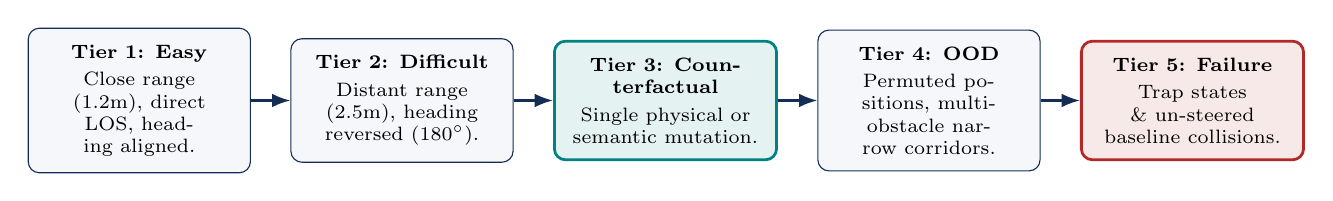
\begin{tikzpicture}[node distance=0.4cm and 0.5cm, auto, >=Latex]
      \tikzstyle{tierbox} = [rectangle, rounded corners, draw=navyblue, fill=lightbg, inner sep=6pt, text width=2.4cm, align=center, font=\scriptsize]
      \tikzstyle{highlightbox} = [rectangle, rounded corners, draw=accentteal, line width=1pt, fill=accentteal!10, inner sep=6pt, text width=2.4cm, align=center, font=\scriptsize]
      \tikzstyle{alertbox} = [rectangle, rounded corners, draw=alertred, line width=1pt, fill=alertred!10, inner sep=6pt, text width=2.4cm, align=center, font=\scriptsize]

      \node[tierbox] (t1) {\textbf{Tier 1: Easy}\\[2pt]Close range (1.2m), direct LOS, heading aligned.};
      \node[tierbox, right=of t1] (t2) {\textbf{Tier 2: Difficult}\\[2pt]Distant range (2.5m), heading reversed ($180^\circ$).};
      \node[highlightbox, right=of t2] (t3) {\textbf{Tier 3: Counterfactual}\\[2pt]Single physical or semantic mutation.};
      \node[tierbox, right=of t3] (t4) {\textbf{Tier 4: OOD}\\[2pt]Permuted positions, multi-obstacle narrow corridors.};
      \node[alertbox, right=of t4] (t5) {\textbf{Tier 5: Failure}\\[2pt]Trap states \& un-steered baseline collisions.};

      \draw[->, thick, navyblue] (t1) -- (t2);
      \draw[->, thick, navyblue] (t2) -- (t3);
      \draw[->, thick, navyblue] (t3) -- (t4);
      \draw[->, thick, navyblue] (t4) -- (t5);
    \end{tikzpicture}
  \end{center}

  \vspace{0.4cm}
  \begin{block}{Role of Failure Demonstrations (Tier 5)}
    \small
    Failure trajectories (e.g., straight-line un-steered collisions and corner traps) provide critical negative exemplars, enabling Sparse Autoencoders (Phase 4) and Causal Scrubbing (Phase 5) to isolate the exact subcircuits responsible for evasive steering.
  \end{block}
\end{frame}

% -----------------------------------------------------------------------------
% Slide 4: The Seven Counterfactual Interventions (E1 - E7)
% -----------------------------------------------------------------------------
\begin{frame}{3. Seven Paired Counterfactual Interventions (E1 -- E7)}
  \textbf{Core Insight:} \textit{Matched pair interventions $(E_0, E_i)$ isolate true relational invariants from superficial visual shortcuts.}

  \vspace{0.2cm}
  \begin{columns}[T]
    \begin{column}{0.52\textwidth}
      \small
      \begin{tabular}{cll}
        \toprule
        \textbf{ID} & \textbf{Physical Mutation} & \textbf{Tested Invariance} \\
        \midrule
        \textbf{E1} & Target position relocated & Preposition meaning ("behind") \\
        \textbf{E2} & Cylinder colored blue/red & Spatial vector decoupled from color \\
        \textbf{E3} & Robot heading $+90^\circ$ & Allocentric spatial orientation \\
        \textbf{E4} & Robot starts in quadrant II & Goal attractor invariance \\
        \textbf{E5} & Obstacle inserted on LOS & Goal identity under detour \\
        \textbf{E6} & Cylinder replaced by box & Shape invariance \\
        \textbf{E7} & Camera pitch altered $+10^\circ$ & Viewpoint robustness \\
        \bottomrule
      \end{tabular}
    \end{column}

    \begin{column}{0.45\textwidth}
      \begin{alertblock}{The Disentanglement Principle}
        \small
        If a latent neuron fires when the target cylinder changes color but the spatial objective is invariant, that neuron encodes \textbf{appearance entanglement}.
        \vspace{0.15cm}

        The E1--E7 suite directly pinpoints which layers disentangle perception from action.
      \end{alertblock}
    \end{column}
  \end{columns}
\end{frame}

% -----------------------------------------------------------------------------
% Slide 5: Disambiguating Coordinate Frames & Perceptions
% -----------------------------------------------------------------------------
\begin{frame}{4. Resolving Fundamental Ambiguities}
  \textbf{Core Insight:} \textit{Four targeted probe suites distinguish coordinate frames and separate optical appearance from kinematic reachability.}

  \vspace{0.2cm}
  \begin{columns}[T]
    \begin{column}{0.48\textwidth}
      \begin{block}{D1: Egocentric vs. Allocentric Left}
        \small
        When facing South ($\theta = -\frac{\pi}{2}$):
        \begin{itemize}
          \item \textbf{Ego Left}: East ($+x_{\text{world}}$).
          \item \textbf{Allocentric Left}: West ($-x_{\text{world}}$).
          \item Distinguishes whether the policy reasons in body or world coordinates.
        \end{itemize}
      \end{block}

      \begin{block}{D2: Retinal Front vs. Object Behind}
        \small
        Moving directly forward reaches "in front", but reaching "behind" requires an active circumnavigation flank.
      \end{block}
    \end{column}

    \begin{column}{0.48\textwidth}
      \begin{block}{D3: Apparent Size vs. Metric Proximity}
        \small
        A $2\times$ larger box at $2\times$ distance subtends the exact same $18.5^\circ$ FOV.
        Probes whether the latent space encodes metric Euclidean distance or 2D image area.
      \end{block}

      \begin{alertblock}{D4: Optical Visibility vs. Reachability}
        \small
        Target is optically visible through a $0.15\,\text{m}$ gap, but the AMR width ($0.26\,\text{m}$) prohibits passage. Probes topological planning.
      \end{alertblock}
    \end{column}
  \end{columns}
\end{frame}

% -----------------------------------------------------------------------------
% Slide 6: Benchmark Dataset Partitioning & Leakage Elimination
% -----------------------------------------------------------------------------
\begin{frame}{5. Partitioning Strategy: Zero Observation Leakage}
  \textbf{Core Insight:} \textit{Splitting strictly by environmental configuration seeds guarantees zero observation or frame leakage across splits.}

  \vspace{0.2cm}
  \begin{columns}[T]
    \begin{column}{0.55\textwidth}
      \begin{block}{The Danger of Frame-Level Random Splits}
        \small
        Randomly shuffling transitions $(o_t, a_t, o_{t+1})$ leaks adjacent video frames across train and test sets, artificially inflating generalization metrics.
      \end{block}

      \vspace{0.15cm}
      \begin{block}{Partitioning by Environment Configuration}
        \small
        Splits are strictly segregated by \textbf{entire scene configurations and random seeds}:
        \begin{itemize}
          \item \textbf{Train Benchmark}: 408 episodes (12,595 transitions).
          \item \textbf{Validation Benchmark}: 96 episodes (2,911 transitions).
          \item \textbf{Held-out Test Benchmark}: 96 episodes (2,885 transitions).
        \end{itemize}
      \end{block}
    \end{column}

    \begin{column}{0.42\textwidth}
      \centering
      \small
      \textbf{Total Benchmark Corpus}\\[4pt]
      \begin{tabular}{lrr}
        \toprule
        \textbf{Dataset Split} & \textbf{Episodes} & \textbf{Frames} \\
        \midrule
        Train Benchmark & 408 & 12,595 \\
        Val Benchmark & 96 & 2,911 \\
        Held-out Test & 96 & 2,885 \\
        Counterfactual (E1-E7) & 350 & 12,250 \\
        Disambiguation & 100 & 3,254 \\
        \midrule
        \textbf{Total Corpus} & \textbf{1,050} & \textbf{33,895} \\
        \bottomrule
      \end{tabular}
      \vspace{0.2cm}
      \footnotesize
      Total Storage: 165.78 MB (Compressed NPZ)
    \end{column}
  \end{columns}
\end{frame}

% -----------------------------------------------------------------------------
% Slide 7: Phase 1 Acceptance Criteria & Verification
% -----------------------------------------------------------------------------
\begin{frame}{6. Phase 1 Verification \& Prerequisites for Phase 2}
  \textbf{Core Insight:} \textit{With 1,050 reproducible episodes across 6 capabilities and 5 tiers, Phase 1 acceptance criteria are fully satisfied.}

  \vspace{0.3cm}
  \begin{block}{Phase 1 Acceptance Criteria Checklist}
    \small
    \begin{itemize}
      \item[\checkmark] \textbf{Reproducible Episodes}: 1,050 episodes generated deterministically ($>100$ per capability).
      \item[\checkmark] \textbf{Controlled Variations}: Controlled variations across position, orientation, color, shape, and obstacles.
      \item[\checkmark] \textbf{Split Separation}: Train, validation, held-out test, counterfactual, and disambiguation splits completely isolated.
      \item[\checkmark] \textbf{Ground-Truth Physical State}: 15-field schema logs exact poses, velocities, and 3D coordinates for mechanistic probing without leakage to models.
      \item[\checkmark] \textbf{Data Integrity}: 0 NaNs, verified tensor dimensions, and complete companion metadata.
    \end{itemize}
  \end{block}

  \vspace{0.2cm}
  \begin{alertblock}{Readiness for Phase 2}
    \small
    The experimental laboratory is fully prepared to execute \textbf{Phase 2: Establish Behavioral Baselines} across Baseline Policy, LeWM, and H-JEPA under identical evaluation seeds.
  \end{alertblock}
\end{frame}

\end{document}
